\documentclass[10pt, letterpaper]{article}

\usepackage[margin=1in]{geometry}
\usepackage[T1]{fontenc}
\usepackage{lmodern}
\usepackage{amsmath, amssymb, amsthm}
\usepackage{booktabs}
\usepackage{graphicx}
\usepackage{xcolor}
\usepackage{hyperref}
\usepackage{enumitem}
\usepackage{caption, subcaption}
\usepackage{multirow}

\title{Ordering Is Not Invariant:\\ The Absence of Permutation Group Structure\\ in Language Model Representations}
\author{Robb Walters}
\date{April 2026}

\begin{document}
\maketitle

\begin{abstract}
We investigate whether transformer language models develop internal representations with permutation group symmetry. Using operator fitting, group relation testing, and representation-theoretic analysis across two scales of Qwen2.5 (0.5B, 1.5B), we find that models are strongly permutation-\emph{sensitive}---linear operators mapping between permuted representations fit 21$\times$ better than chance---but exhibit zero group-algebraic structure. Composition errors for $S_3$ operators fall in the no-structure regime ($\approx 1.0$), far from the ${<}\,0.1$ expected under true group structure. This null result holds across all layers, in PCA subspaces, in sparse autoencoder feature bases, and at both model scales. A positive control on synthetic data with exact group structure confirms the pipeline would detect it if present. We extend these findings to fact-level permutations, showing that reordering the same facts changes model representations 35--60\% as much as presenting entirely different facts, with next-token predictions changing 30\% of the time. We argue this reflects a fundamental property: local optimization under next-token prediction learns \emph{functional} equivariance (correct outputs under transformation) without \emph{structural} equivariance (group representations in latent space). This has implications for synthetic data generation, where the implicit assumption that semantic content is order-invariant may destroy information the model has learned about salience and discourse structure.
\end{abstract}

%----------------------------------------------------------------------
\section{Introduction}
\label{sec:intro}

Symmetry has been among the most powerful organizing principles in science. In physics, the discovery that physical laws are invariant under specific group actions---translations, rotations, gauge transformations---has led to conservation laws, unified theories, and deep structural understanding \cite{noether1918, weyl1952}. In machine learning, the geometric deep learning program has shown that building symmetry into neural network architectures through equivariant layers improves sample efficiency and generalization \cite{bronstein2021geometric, cohen2016group}.

A natural question arises: do neural networks trained on data with implicit symmetries develop \emph{internal} representations that respect those symmetries, even without explicit architectural constraints? Recent work on Group Crosscoders \cite{gorton2024group} provides a positive answer for vision: a convolutional network trained on natural images develops approximate dihedral group ($D_{32}$) equivariance in its early vision layers. And small transformers trained on modular arithmetic learn explicit circular representations that embed the group structure of addition \cite{nanda2023grokking}. But do such structures emerge in general-purpose language models trained on natural text?

We ask whether language model representations of permuted entities or reordered facts carry the algebraic structure of the symmetric group $S_n$. If ``Alice gave Bob the book'' and ``Bob gave Alice the book'' produce activations related by a linear operator $W_\pi$, do these operators compose as group elements---does $W_{\pi_1} W_{\pi_2} \approx W_{\pi_1 \circ \pi_2}$?

Our central finding is that models achieve \emph{functional} equivariance without \emph{structural} equivariance. The model's outputs transform correctly under permutation (swap Alice and Bob, the completion swaps), but the internal operators implementing these transformations do not satisfy group composition laws. The model has learned a lookup table, not an algebra. We argue this distinction---between getting the right answer and having the right internal structure---is fundamental to understanding what local optimization can and cannot discover.

This question has practical significance. Modern approaches to synthetic data generation, such as the Simula framework \cite{davidson2026simula}, decompose data domains into independent factors sampled from hierarchical taxonomies. This product-space decomposition implicitly assumes that reordering content is semantically neutral. If language models have learned that ordering encodes information---salience, narrative priority, discourse structure---then synthetic data approaches that scramble ordering may destroy signal the model has learned to use.

Our contributions are:
\begin{enumerate}[itemsep=2pt]
    \item A comprehensive empirical demonstration that language model representations are permutation-\emph{sensitive} but not permutation-\emph{equivariant}: linear operators fit well individually but fail all group composition tests ($S_3$ relation errors $\approx 1.0$, in the no-structure regime).
    \item Positive controls and random baselines establishing that the detection pipeline works (relation errors $\to 0$ on synthetic group-structured data) and that the null result is not an artifact of insufficient signal.
    \item Evidence that fact-level reordering is \emph{not} a symmetry of the model's world representation: reordering the same facts changes activations 35--60\% as much as presenting entirely different facts, with next-token predictions changing 30\% of the time.
    \item A conceptual framework distinguishing \emph{functional equivariance} from \emph{structural equivariance}, explaining why the former is achievable without the latter under local optimization.
\end{enumerate}

%----------------------------------------------------------------------
\section{Background}
\label{sec:background}

\subsection{Group Representations and Equivariance}

A \emph{representation} of a group $G$ on a vector space $V$ is a homomorphism $\rho: G \to GL(V)$---a map assigning to each group element $g$ an invertible linear transformation $\rho(g)$ such that $\rho(g_1 g_2) = \rho(g_1)\rho(g_2)$. A function $f: V \to W$ is \emph{equivariant} with respect to representations $\rho_V, \rho_W$ if $f(\rho_V(g) \cdot x) = \rho_W(g) \cdot f(x)$ for all $g \in G, x \in V$.

The symmetric group $S_n$ consists of all permutations of $n$ elements. $S_3$ has order 6 and is generated by a transposition $s = (0\;1)$ and a 3-cycle $r = (0\;1\;2)$ with presentation $\langle s, r \mid s^2 = e, r^3 = e, srs = r^{-1} \rangle$. Its irreducible representations are: the trivial representation (1D, all elements $\to 1$), the sign representation (1D, even permutations $\to +1$, odd $\to -1$), and the standard representation (2D).

We distinguish two notions of equivariance in neural networks:
\begin{itemize}[itemsep=2pt]
    \item \textbf{Functional equivariance}: the model's \emph{output} transforms correctly under input permutations. If we swap Alice and Bob in a prompt, the model's completion swaps accordingly.
    \item \textbf{Structural equivariance}: the model's \emph{internal representations} carry group structure. The operators relating permuted activations satisfy group composition laws.
\end{itemize}
A model can achieve functional equivariance without structural equivariance---by implementing a lookup table rather than an algebra.

\subsection{Prior Work}

\paragraph{Group structure in neural networks.} Gorton\ \cite{gorton2024group} introduced Group Crosscoders, training sparse autoencoders on concatenated activations from transformed inputs to discover symmetry structure. Applied to InceptionV1, they found approximate $D_{32}$ equivariance in early vision features. Nanda et al.\ \cite{nanda2023grokking} showed that small transformers trained on modular addition learn explicit group structure, embedding inputs as rotations on a circle. These positive results establish that group structure \emph{can} emerge---but in both cases the group structure \emph{is} the task (rotation of edges, modular arithmetic). Our work tests whether group structure emerges when the task does not require it.

\paragraph{Geometric deep learning.} Bronstein et al.\ \cite{bronstein2021geometric} survey the program of building symmetry into network architectures. Cohen and Welling \cite{cohen2016group} showed that group equivariant CNNs improve generalization. Xu et al.\ \cite{xu2024permutation} proved that vanilla transformers possess inter- and intra-token permutation equivariance---an architectural property distinct from learned representational structure.

\paragraph{Linear representations in LLMs.} Park et al.\ \cite{park2024linear} formalized the linear representation hypothesis using counterfactual semantics, showing that high-level concepts are represented as linear directions in LLM representation spaces. Our operator fitting approach is consistent with this framework: we test whether permutation-induced changes are linear (they are) and whether the resulting linear operators have algebraic structure (they do not).

\paragraph{Position sensitivity in LLMs.} Liu et al.\ \cite{liu2024lost} showed that LLM performance follows a U-shaped curve with information position---best for information at the beginning and end of the context, degrading for information in the middle. This ``lost in the middle'' finding provides independent evidence that ordering matters to LLMs and suggests a mechanistic explanation (attention bias) for the recency effects we observe in our fact-ordering experiments.

\paragraph{Synthetic data generation.} Davidson et al.\ \cite{davidson2026simula} introduced Simula, decomposing data generation into coverage, complexity, and quality axes via hierarchical taxonomies sampled as a product space $\mathcal{T}_0 \times \mathcal{T}_1 \times \cdots \times \mathcal{T}_K$. While Simula's mixing strategies partially address factor dependencies, the underlying product-space assumption---that factors are independently combinable---is a form of exchangeability assumption that our results call into question.

\paragraph{Information structure in linguistics.} The pragmatics literature has long established that utterance ordering encodes topic-focus structure, givenness, and information status \cite{krifka2008, lambrecht1994}. Given information typically precedes new information; propositions closest to the discourse topic are uttered first \cite{vandijk1977}. Our empirical findings are consistent with these linguistic principles.

%----------------------------------------------------------------------
\section{Methods}
\label{sec:methods}

\subsection{Models and Setup}

We study Qwen2.5-0.5B (24 layers, $d_\text{model} = 896$) and Qwen2.5-1.5B (28 layers, $d_\text{model} = 1536$), both base (non-instruct) models \cite{qwen2025}. Activations are captured using TransformerLens \cite{nanda2022transformerlens} at the residual stream (post-block) of every layer, at the last token position. All experiments run on a single Apple M3 Ultra (96GB unified memory) using the MPS backend. Random seeds are fixed at 42 for all stochastic operations.

\subsection{Permutation Prompt Design}

We construct two types of permutation experiments:

\paragraph{Entity-level permutations.} Fixed sentence templates with named entity slots, e.g., ``\{e0\} and \{e1\} entered the room. The first to enter was''. Entity names (Alice, Bob, Carol) are chosen for single-token encoding and matched tokenization length. For $S_3$, we generate all 6 permutations of 3-entity templates across 10 templates and 10 entity sets, yielding 100 samples per non-identity permutation.

\paragraph{Fact-level permutations.} Multi-sentence sequences where each sentence is an independent fact. We generate all $n!$ orderings and compare activations and predictions. We use 15 fact sets each for $S_2$ (2-fact) and $S_3$ (3-fact) sequences, including examples spanning urgency levels (e.g., ``The room is on fire.'' alongside ``It is Wednesday.'').

\subsection{Operator Fitting}

For each permutation $\pi \in S_n$ (excluding identity), we collect paired activations $(h(x), h(\pi \cdot x))$ across many prompts and fit a linear operator $W_\pi$ via least-squares regression:
\begin{equation}
    W_\pi = \arg\min_W \|W \cdot H_\text{base}^T - H_\text{perm}^T\|_F^2
\end{equation}
where $H_\text{base}, H_\text{perm} \in \mathbb{R}^{n \times d}$ are matrices of base and permuted activations. We use an 80/20 train/test split and report test-set relative error $\|Y - \hat{Y}\|_F / \|Y\|_F$ and cosine similarity.

\subsection{Group Relation Testing}

Given fitted operators $\{W_\pi\}$, we test the $S_3$ presentation relations:
\begin{align}
    W_s^2 &\approx I \quad \text{(transposition is involution)} \\
    W_r^3 &\approx I \quad \text{(3-cycle cubes to identity)} \\
    W_s W_r W_s &\approx W_r^{-1} = W_r^2 \quad \text{(conjugation relation)}
\end{align}
and full composition closure: $W_{\pi_1} W_{\pi_2} \approx W_{\pi_1 \circ \pi_2}$ for all pairs. We report relative error $\|LHS - RHS\|_F / \|RHS\|_F$.

\subsection{Controls}

\paragraph{Positive control.} We construct synthetic activations with exact $S_3$ group structure: random base vectors $x \in \mathbb{R}^d$ mapped by exact representation matrices $W_\pi$ (the combined trivial + sign + standard irrep, embedded in $d = 10$ dimensions via random orthogonal rotation) plus calibrated Gaussian noise. The positive control uses a well-conditioned system ($n = 200 > d = 10$). While the real model operates at $d = 896$ with $n = 100$ samples (underdetermined), the real model's low test errors (0.08) demonstrate that the system is effectively well-conditioned for neural activations, which are low-rank. The positive control validates the group relation testing; the real model's operator fit quality validates the linear algebra.

\paragraph{Random baseline.} We fit operators on \emph{shuffled} prompt pairs---base activations from one prompt paired with ``permuted'' activations from an unrelated prompt---averaged over 5 independent shuffles. This establishes the chance-level floor for both fit quality and group relation errors.

\subsection{Additional Analyses}

\paragraph{Subspace search.} PCA on activation differences $\Delta h = h(\pi \cdot x) - h(x)$ to find a permutation-sensitive subspace. Operators fitted and group relations tested in projected subspaces of dimension 3--200.

\paragraph{Irreducible representation search.} Direct optimization for the sign representation (direction $v$ with $W_s v \approx -v$, $W_r v \approx +v$) and the standard 2D irrep.

\paragraph{SAE feature-space analysis.} Sparse autoencoders \cite{bricken2023monosemanticity} (8$\times$ expansion, 5M training tokens, $L_1$ coefficient 5.0, learning rate $3 \times 10^{-4}$) trained on layers 0 and 21. Activations encoded through the SAE, operators fitted and group relations tested in the sparse feature basis.

\paragraph{Fact-order analysis.} For fact-level permutations: (1) relative activation distance between reorderings vs.\ between different fact sets; (2) KL divergence and top-1 agreement of next-token predictions; (3) group structure testing on fact-reordering operators.

%----------------------------------------------------------------------
\section{Results}
\label{sec:results}

\subsection{Entity-Level Permutations: Strong Signal, No Structure}

\paragraph{Behavioral validation.} The model reliably tracks entity permutations at the output level: swapping Alice and Bob in ``\{e0\} and \{e1\} entered the room. The first to enter was'' shifts the top-1 prediction from ``Alice'' to ``Bob'' with comparable confidence. KL divergences between identity and permuted outputs range from 0.15 to 2.1 across templates, confirming functional equivariance.

\paragraph{Activation alignment.} Operator fit quality follows a U-shaped layer profile (Figure~\ref{fig:layer_profile}a, Table~\ref{tab:alignment}). Early layers (0--2) fit best, with test-set relative errors as low as 0.08 for the 0.5B model. Middle layers (10--16) fit worst ($\sim$0.43). Late layers (20--22) show a secondary peak ($\sim$0.26). The 1.5B model exhibits the same pattern (best at layer 0, test error 0.12). The permutation signal is strongly linearly predictable at all layers.

\begin{figure}[t]
\centering

\includegraphics[width=\textwidth]{figures/fig1_layer_profile.pdf}
\caption{Layer-by-layer analysis for $S_3$ entity permutations. (a)~Operator fit quality (test-set relative error) follows a U-shaped profile: best at early and late layers. Both model scales show the same pattern. (b)~Group relation errors remain $\approx 1.0$ at every layer regardless of fit quality, indicating no algebraic structure. The gray dotted line at 1.0 represents the error expected from unrelated operators. The green region (${<}\,0.1$) indicates where errors would fall if true group structure were present, as validated by our positive control (Figure~\ref{fig:positive_control}).}
\label{fig:layer_profile}
\end{figure}

\begin{table}[t]
\centering
\caption{Operator fit quality and group relation errors for $S_3$ at matched relative depths. Layers are selected so that the relative position (layer/total) is comparable across model scales. An error of $\approx 1.0$ indicates no better than random composition; a positive control at comparable test error yields errors of 0.04--0.06.}
\label{tab:alignment}
\small
\begin{tabular}{@{}lcccccccc@{}}
\toprule
& & \multicolumn{3}{c}{Qwen2.5-0.5B} & \multicolumn{4}{c}{Qwen2.5-1.5B} \\
\cmidrule(lr){3-5} \cmidrule(lr){6-9}
Depth & Layer & Test Err & $s^2\!=\!e$ & $r^3\!=\!e$ & Layer & Test Err & $s^2\!=\!e$ & $r^3\!=\!e$ \\
\midrule
0.0  & 0  & 0.078 & 1.023 & 1.094 & 0  & 0.123 & 0.987 & 1.006 \\
0.2  & 5  & 0.249 & 1.040 & 1.040 & 6  & 0.230 & 1.012 & 1.018 \\
0.4  & 10 & 0.408 & 1.021 & 1.020 & 10 & 0.323 & 1.012 & 1.020 \\
0.7  & 16 & 0.429 & 1.031 & 1.031 & 18 & 0.479 & 1.011 & 1.009 \\
0.9  & 21 & 0.258 & 1.015 & 1.024 & 25 & 0.336 & 1.006 & 1.009 \\
\bottomrule
\end{tabular}
\end{table}

\paragraph{Group relations: the null result.} Despite good individual operator fits, all $S_3$ presentation relations fail (Figure~\ref{fig:layer_profile}b, Table~\ref{tab:alignment}). Relation errors are $\approx 1.0$ at every layer, for both model scales---firmly in the no-structure regime, and far from the ${<}\,0.1$ that the positive control shows is achievable when group structure is present. The random baseline confirms that the permutation signal is real (operators fit 21$\times$ better than shuffled pairs) but the algebraic structure is not.

\paragraph{The pattern is robust.} We tested every natural place group structure might hide. In PCA subspaces (3--200D), the best result (layer 0, dim 3) achieves $s^2 = e$ error 0.09 but $r^3 = e$ still fails at 0.73. No sign representation or standard 2D irrep was detected at any layer via direct optimization. In the SAE feature basis, group relations are \emph{worse} than raw activation space (errors 1--34$\times$). Eigenvalue analysis reveals transposition operators are rank-deficient projections ($\det \approx 0$, eigenvalues near $+1$, none near $-1$), not reflections. The 1.5B model shows identical patterns across all 28 layers (Table~\ref{tab:alignment}).

\subsection{Controls}

\paragraph{Positive control.} Synthetic activations with exact $S_3$ representations embedded in $\mathbb{R}^{10}$ yield relation errors scaling linearly with noise (Figure~\ref{fig:positive_control}, Table~\ref{tab:positive}). At $\sigma = 0$ errors are numerically zero; at $\sigma = 0.1$ (comparable real-model test error) they are $\sim$0.05. The real model's errors ($\sim$1.0) correspond to the regime where group structure is completely destroyed ($\sigma \geq 1.0$). This confirms the pipeline works and that the null result is genuine.

\begin{figure}[t]
\centering
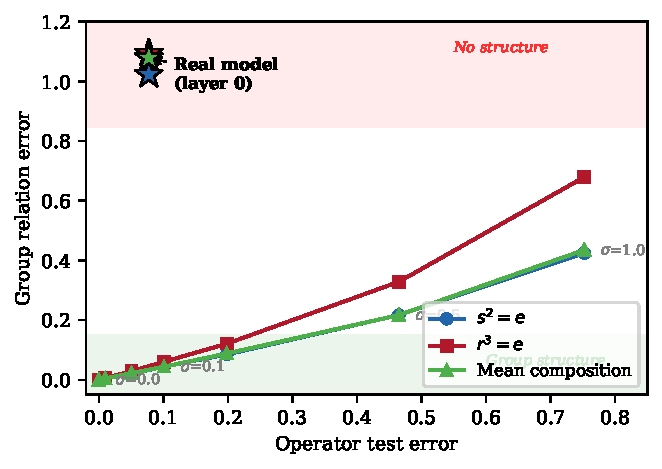
\includegraphics[width=0.65\textwidth]{figures/fig2_positive_control.pdf}
\caption{Positive control: group relation errors vs.\ operator test error for synthetic data with exact $S_3$ structure at varying noise levels. Lines show the calibration curve; stars mark the real model (layer 0). The real model sits in the ``no structure'' region (top) despite having low test error (left)---a pattern impossible under true group structure.}
\label{fig:positive_control}
\end{figure}

\begin{table}[t]
\centering
\caption{Positive control: $S_3$ group relation errors in synthetic data with exact group structure at varying noise levels ($d = 10$, $n = 200$ samples). Compare to real model errors of $\approx 1.0$.}
\label{tab:positive}
\small
\begin{tabular}{@{}lccccc@{}}
\toprule
Noise $\sigma$ & Test Err & $s^2\!=\!e$ & $r^3\!=\!e$ & $srs\!=\!r^{-1}$ & Composition \\
\midrule
0.00 & 0.000 & 0.000 & 0.000 & 0.000 & 0.000 \\
0.01 & 0.010 & 0.005 & 0.006 & 0.006 & 0.004 \\
0.10 & 0.101 & 0.045 & 0.061 & 0.060 & 0.044 \\
0.50 & 0.465 & 0.217 & 0.329 & 0.290 & 0.217 \\
1.00 & 0.752 & 0.425 & 0.679 & 0.631 & 0.435 \\
\midrule
\multicolumn{6}{l}{\textit{Real model (layer 0):} 0.078 test err, but $\sim$1.0 relation errors} \\
\bottomrule
\end{tabular}
\end{table}

\paragraph{Random baseline.} At layer 0, shuffled-pair operators fit with test error $1.68$ (vs.\ $0.08$ for real pairs---a 21$\times$ ratio), confirming the permutation signal is genuine. Group relation errors from shuffled pairs are much larger ($s^2 = e$: 36.9, $r^3 = e$: 158) than from real pairs ($\sim$1.0). However, both are far above the ${<}\,0.1$ threshold that indicates group structure. The real model's relation errors, while lower than random, are $\sim$1.0---firmly in the no-structure regime.

\subsection{Fact-Level Permutations: Ordering Encodes Information}

\paragraph{Activation distance.} Reordering the same facts changes last-token activations substantially (Figure~\ref{fig:fact_distances}, Table~\ref{tab:facts}). The within-set relative distance (same facts, different order) averages 35--60\% of the between-set distance (entirely different facts). This ratio is stable across layers and consistent for 2-fact and 3-fact sequences. The model does \emph{not} treat fact-sets as permutation-invariant.

\begin{figure}[t]
\centering
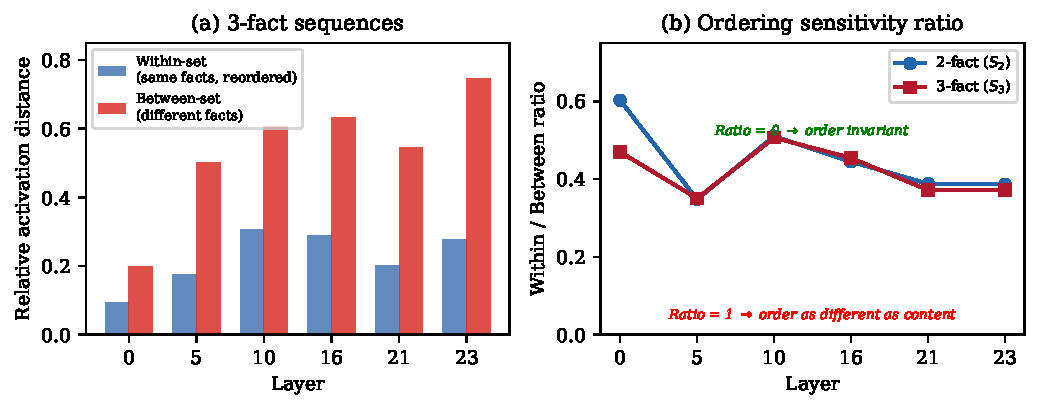
\includegraphics[width=\textwidth]{figures/fig4_fact_distances.pdf}
\caption{Impact of fact reordering on model representations. (a)~Absolute activation distances for 3-fact sequences: reordering the same facts (blue) shifts representations 35--50\% as much as entirely different facts (red). (b)~The within/between ratio is stable at 0.35--0.50 across layers for both 2-fact and 3-fact sequences, far from 0 (order invariance).}
\label{fig:fact_distances}
\end{figure}

\begin{table}[t]
\centering
\caption{Impact of fact reordering on model representations (3-fact sequences, $\pm$ one standard deviation across pairwise comparisons). Ratio $\ll 1$ would indicate permutation invariance; observed ratios of 0.35--0.50 show ordering substantially affects representations.}
\label{tab:facts}
\small
\begin{tabular}{@{}lccc@{}}
\toprule
Layer & Within ($\pm$ SD) & Between ($\pm$ SD) & Ratio \\
\midrule
0  & $0.094 \pm 0.055$ & $0.200 \pm 0.067$ & 0.47 \\
5  & $0.176 \pm 0.079$ & $0.501 \pm 0.111$ & 0.35 \\
10 & $0.307 \pm 0.124$ & $0.606 \pm 0.109$ & 0.51 \\
21 & $0.203 \pm 0.099$ & $0.545 \pm 0.107$ & 0.37 \\
23 & $0.277 \pm 0.144$ & $0.745 \pm 0.120$ & 0.37 \\
\bottomrule
\end{tabular}
\end{table}

\paragraph{Behavioral impact.} Next-token predictions change meaningfully with fact order: top-1 agreement is only 67\% for 2-fact and 71\% for 3-fact sequences (Table~\ref{tab:behavioral}). Mean KL divergence is $0.355 \pm 0.355$ ($S_2$) and $0.285 \pm 0.249$ ($S_3$). The high variance reflects that some fact sets are more order-sensitive than others, but the mean effect is substantial. For 3-fact sequences, even permutations (3-cycles) produce larger KL divergence ($0.366$) than odd permutations (transpositions, $0.231$), consistent with the idea that pairwise swaps are more ``natural'' linguistic operations than ternary rotations.

\begin{table}[t]
\centering
\caption{Behavioral impact of fact reordering ($\pm$ SD across fact sets). Top-1 agreement below 100\% indicates the model's most likely next token changes when facts are reordered. For $S_3$, even permutations (3-cycles) cause larger distributional shifts than odd (transpositions).}
\label{tab:behavioral}
\small
\begin{tabular}{@{}lccc@{}}
\toprule
& Mean KL ($\pm$ SD) & Top-1 Agreement & Even KL / Odd KL \\
\midrule
2-fact ($S_2$) & $0.355 \pm 0.355$ & 66.7\% & --- \\
3-fact ($S_3$) & $0.285 \pm 0.249$ & 70.7\% & 0.366 / 0.231 \\
\bottomrule
\end{tabular}
\end{table}

\paragraph{Case study.} Consider three facts of varying urgency: (F)~``The room is on fire.'' (R)~``I am sitting at my desk researching internal representations in LLMs.'' (W)~``It is Wednesday.'' The KL divergence matrix across all 6 orderings (Figure~\ref{fig:kl_heatmap}) reveals clear block structure: orderings ending with the same fact produce similar predictions (KL $= 0.026$ between F-W-R and W-F-R, both ending with the research fact), while orderings ending with different facts diverge substantially (KL $= 0.35$ between F-R-W and R-W-F). The model attends most to the \emph{last-mentioned} fact---a recency effect consistent with the ``lost in the middle'' phenomenon \cite{liu2024lost}, not a symmetry.

\begin{figure}[t]
\centering
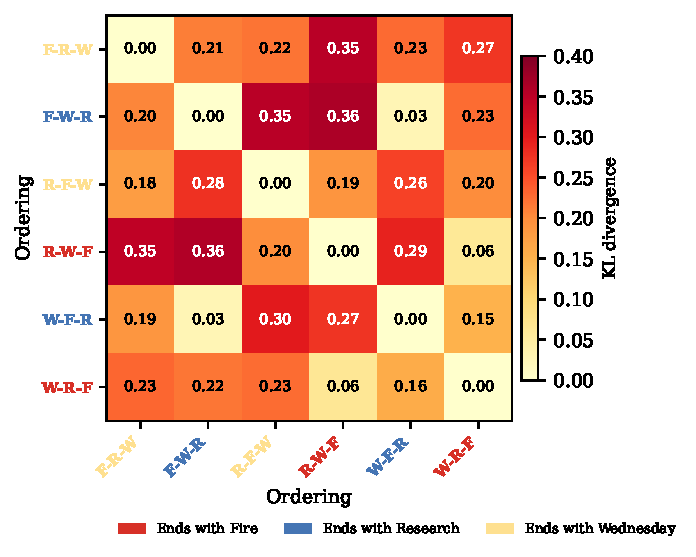
\includegraphics[width=0.65\textwidth]{figures/fig3_kl_heatmap.pdf}
\caption{KL divergence between next-token distributions for all 6 orderings of three facts: ``The room is on fire'' (F), ``I am researching LLM representations'' (R), ``It is Wednesday'' (W). Orderings sharing the same final fact cluster together (block structure), revealing a recency effect. Tick labels are colored by final fact.}
\label{fig:kl_heatmap}
\end{figure}

\paragraph{Group structure.} Fact-reordering operators show the same null result as entity permutations: good individual fits (test error 0.13 at layer 0) but $s^2 = e \approx 0.99$, $r^3 = e \approx 1.00$, composition errors $\approx 0.7$--$0.8$. The pattern generalizes: \emph{no} permutation operation on text---whether entity swaps or fact reordering---induces group-structured representations.

%----------------------------------------------------------------------
\section{Discussion}
\label{sec:discussion}

\subsection{Why No Group Structure?}

Three candidate explanations compete:

\paragraph{(A) The territory.} Idea space does not have $S_n$ symmetry. Ordering genuinely encodes information---salience, temporal priority, narrative frame. The model correctly learned the world's asymmetry. This is supported by our fact-reordering results and by the pragmatics literature on information structure \cite{krifka2008, lambrecht1994}.

\paragraph{(B) The map.} Transformers cannot learn group structure even if it exists. But this is refuted by positive cases: Group Crosscoders \cite{gorton2024group} find approximate $D_{32}$ in vision, and Nanda et al.\ \cite{nanda2023grokking} show transformers learn explicit circular representations for modular arithmetic. The architecture is capable; the question is whether the data and task demand it.

\paragraph{(C) The reward.} Next-token prediction does not incentivize algebraic coherence. Composing permutation operators is never required for correct prediction. A per-permutation linear map has more degrees of freedom than a group-constrained representation, making it easier to fit from limited data---though it sacrifices the compositional generalization that group structure would provide. Since next-token prediction never tests compositional generalization over permutations, the unconstrained solution dominates. Notably, in both positive cases (vision, modular arithmetic), the group structure \emph{is} the task---rotation of visual features, cyclic addition. For natural language, permutation structure is incidental to prediction.

An additional factor may be superposition \cite{elhage2022superposition}: if the model represents permutation information in superposition with other features, interference between compressed representations would prevent operators from satisfying exact algebraic relations even if the underlying computation has group-like structure.

The likely answer combines (A) and (C): the symmetry is not present in natural language, \emph{and} the training objective would not reward learning it even in domains where it exists. Group structure in representations is not free---it requires either architectural inductive bias, data with genuine symmetry, or an objective that rewards compositional generalization over group orbits.

\subsection{Functional vs.\ Structural Equivariance}

Our models achieve functional equivariance: swapping Alice and Bob reliably produces a swapped completion. But they do not achieve structural equivariance: the internal operators implementing this swap do not compose as a group. The model has learned a \emph{lookup table}, not an \emph{algebra}. In physics, discovering that functional regularities arise from structural symmetries required stepping outside the local optimization landscape---a contribution of theoretical reasoning, not of the optimization process itself.

\subsection{Implications for Synthetic Data Generation}

Our results have three levels of implication for synthetic data design:

\paragraph{Level 1: Fact ordering is not a nuisance variable.} Reordering the same facts changes model predictions 30\% of the time (top-1 disagreement). If synthetic training data presents facts in arbitrary order, it generates examples with different implicit salience signals. This is directly measurable and directly actionable.

\paragraph{Level 2: Product-space decomposition has blind spots.} Frameworks like Simula \cite{davidson2026simula} decompose data domains as $\mathcal{T}_0 \times \mathcal{T}_1 \times \cdots \times \mathcal{T}_K$ and sample factors independently. While Simula's mixing strategies mitigate some illogical combinations, the fundamental assumption that factors can be freely recombined does not account for the ordering and salience structure that trained models have learned. Our results show that ordering creates correlations between factors that product-space sampling misses.

\paragraph{Level 3: Symmetry is earned, not assumed.} In physics, symmetries are \emph{discoveries}---insights that required stepping outside local reward signals. In synthetic data generation, symmetries are \emph{assumptions}---choices about what transformations preserve meaning. Our work suggests caution about assuming symmetries that have not been empirically verified. The Group Crosscoders result shows that group structure \emph{does} emerge when the data has physical symmetry. Our result shows it does \emph{not} emerge for linguistic permutations. The lesson: verify, don't assume.

%----------------------------------------------------------------------
\section{Limitations}
\label{sec:limitations}

We tested only small symmetric groups ($S_2$, $S_3$); larger groups or continuous symmetries may behave differently. Our experiments use two models from the same family (Qwen2.5); architecture-specific effects are possible. The fact-level permutation experiments use relatively simple multi-sentence sequences; more complex discourse structures may show different patterns. We did not test whether training with permutation-augmented data would \emph{induce} group structure, nor did we directly compare model performance when fine-tuned on ordered vs.\ shuffled synthetic data. Our positive control uses low-dimensional spaces ($d = 10$); while we argue the real model's low test errors validate the high-dimensional linear algebra, a high-dimensional positive control with realistic activation manifolds would strengthen this argument.

%----------------------------------------------------------------------
\section{Conclusion}
\label{sec:conclusion}

Transformer language models develop permutation-sensitive but not permutation-equivariant representations. This is not a failure of the model---it reflects the structure of the task and the data. Idea space does not have $S_n$ symmetry; fact ordering encodes salience, priority, and narrative structure. Local optimization under next-token prediction correctly learns this asymmetry without discovering the group-theoretic abstractions that would be needed for compositional generalization over permutations.

For synthetic data generation, this means that treating semantic content as order-invariant is an empirical assumption that may not hold. Ordering should be treated as a meaningful dimension of the data---a carrier of information about salience and discourse structure---rather than a nuisance variable to be averaged out.

More broadly, our results illustrate that the presence or absence of symmetry in neural representations is diagnostic of the presence or absence of symmetry in the data domain. Group Crosscoders find rotational structure in vision because rotational symmetry is real. We find no permutation structure in language because permutation symmetry is not. Symmetry in representations is earned by symmetry in the world---it is not a universal gift of neural network optimization.

Natural extensions include training models on permutation-augmented data to test whether group structure can be induced, extending to other symmetries in language (negation, tense shifts), and investigating whether biological visual systems show the rotational group structure that artificial vision models exhibit.

\paragraph{Code availability.} All code and experimental scripts are publicly available at \url{https://github.com/rjwalters/latent-space-symmetries}.

%----------------------------------------------------------------------
\begin{thebibliography}{99}

\bibitem{noether1918}
E.~Noether, ``Invariante Variationsprobleme,'' \textit{Nachr.\ d.\ K\"onig.\ Gesellsch.\ d.\ Wiss.\ zu G\"ottingen}, pp.~235--257, 1918.

\bibitem{weyl1952}
H.~Weyl, \textit{Symmetry}. Princeton University Press, 1952.

\bibitem{bronstein2021geometric}
M.~M.~Bronstein, J.~Bruna, T.~Cohen, and P.~Veli\v{c}kovi\'{c}, ``Geometric deep learning: Grids, groups, graphs, geodesics, and gauges,'' \textit{arXiv preprint arXiv:2104.13478}, 2021.

\bibitem{cohen2016group}
T.~Cohen and M.~Welling, ``Group equivariant convolutional networks,'' in \textit{Proc.\ ICML}, 2016.

\bibitem{gorton2024group}
L.~Gorton, ``Group crosscoders for mechanistic analysis of symmetry,'' \textit{arXiv preprint arXiv:2410.24184}, 2024.

\bibitem{nanda2023grokking}
N.~Nanda, L.~Chan, T.~Lieberum, J.~Smith, and J.~Steinhardt, ``Progress measures for grokking via mechanistic interpretability,'' in \textit{Proc.\ ICLR}, 2023.

\bibitem{davidson2026simula}
T.~R.~Davidson, B.~Seguin, E.~Bacis, C.~Ilharco, and H.~Harkous, ``Reasoning-driven synthetic data generation and evaluation,'' \textit{Trans.\ Machine Learning Research}, 2026.

\bibitem{park2024linear}
K.~Park, Y.~J.~Choe, and V.~Veitch, ``The linear representation hypothesis and the geometry of large language models,'' in \textit{Proc.\ ICML}, 2024.

\bibitem{xu2024permutation}
H.~Xu, L.~Xiang, H.~Ye, D.~Yao, P.~Chu, and B.~Li, ``Permutation equivariance of transformers and its applications,'' in \textit{Proc.\ CVPR}, 2024.

\bibitem{liu2024lost}
N.~F.~Liu, K.~Lin, J.~Hewitt, A.~Paranjape, M.~Bevilacqua, F.~Petroni, and P.~Liang, ``Lost in the middle: How language models use long contexts,'' \textit{Trans.\ Assoc.\ Comput.\ Linguistics}, vol.~12, pp.~157--173, 2024.

\bibitem{bricken2023monosemanticity}
T.~Bricken, A.~Templeton, J.~Batson, et~al., ``Towards monosemanticity: Decomposing language models with dictionary learning,'' Anthropic, 2023.

\bibitem{elhage2022superposition}
N.~Elhage, T.~Hume, C.~Olsson, et~al., ``Toy models of superposition,'' \textit{arXiv preprint arXiv:2209.10652}, 2022.

\bibitem{nanda2022transformerlens}
N.~Nanda, ``TransformerLens,'' 2022. \url{https://github.com/TransformerLensOrg/TransformerLens}

\bibitem{qwen2025}
Qwen Team, ``Qwen2.5 Technical Report,'' \textit{arXiv preprint arXiv:2412.15115}, 2024.

\bibitem{krifka2008}
M.~Krifka, ``Basic notions of information structure,'' \textit{Acta Linguistica Hungarica}, vol.~55, pp.~243--276, 2008.

\bibitem{lambrecht1994}
K.~Lambrecht, \textit{Information Structure and Sentence Form}. Cambridge University Press, 1994.

\bibitem{vandijk1977}
T.~A.~van Dijk, ``The pragmatics of discourse,'' in \textit{Text and Context}, 1977.

\end{thebibliography}

\end{document}
